%% %% %% %%
%%
%% Parte A de la práctica
%%
%% %% %% %%

\documentclass[../procedimientos.tex]{subfiles}
\graphicspath{{\subfix{../../images/}}}

\begin{document}
\clearpage
\subsection{Parte A}
\subsubsection{Instrucciones}
\begin{em}
  Construir de manera gráfica las siguientes compuertas lógicas y simularlas 
  dentro de la plataforma Quartus.
  \begin{itemize}
      \item AND
      \item OR
      \item NOT
      \item XOR (y su forma expandida)
  \end{itemize}
\end{em}

\subsubsection{Análisis}
Antes de comenzar a realizar esta sección, es importante tener muy presente el 
comportamiento de cada una de las compuertas con la finalidad de comprobar de 
forma satisfactoria el resultado de la actividad. La tabla de verdad de cada 
una de las compuertas se muestra a continuación:
\begin{table}[h!]
  \caption{Tablas de verdad (Sección A)}
  \label{tab:a_tv}
  \centering
  \begin{subtable}[t]{0.25\linewidth} % Compuerta AND
    \centering
    \label{tab:comp_and}
    \begin{tabular}{|c c|c|}
      \hline
      $A$ & $B$ & $A \cdot B$\\
      \hline
      0 & 0 & 0\\
      0 & 1 & 0\\
      1 & 0 & 0\\
      1 & 1 & 1\\
      \hline
    \end{tabular}
    \caption{Compuerta AND}
  \end{subtable}
  \begin{subtable}[t]{0.25\linewidth} % Compuerta OR
    \centering
    \label{tab:comp_or}
    \begin{tabular}{|c c|c|}
      \hline
      $A$ & $B$ & $A + B$\\
      \hline
      0 & 0 & 0\\
      0 & 1 & 1\\
      1 & 0 & 1\\
      1 & 1 & 1\\
      \hline
    \end{tabular}
    \caption{Compuerta OR}
  \end{subtable}
  \begin{subtable}[t]{0.20\linewidth} % Compuerta NOT
    \centering
    \label{tab:comp_not}
    \begin{tabular}{|c|c|}
      \hline
      $A$ & $\nt{A}$\\
      \hline
      0 & 1\\
      1 & 0\\
      \hline
    \end{tabular}
    \caption{Compuerta NOT}
  \end{subtable}
  \begin{subtable}[t]{0.25\linewidth} % Compuerta XOR
    \centering
    \label{tab:comp_xor}
    \begin{tabular}{|c c|c|}
      \hline
      $A$ & $B$ & $A \oplus B$\\
      \hline
      0 & 0 & 0\\
      0 & 1 & 1\\
      1 & 0 & 1\\
      1 & 1 & 0\\
      \hline
    \end{tabular}
    \caption{Compuerta XOR}
  \end{subtable}
\end{table}

De igual forma, se pueden comporbar la siguiente equivalencia entre las 
operaciones lógicas XOR, AND y OR:
\begin{equation}
  A \oplus B = \nt{A} \cdot B + A \cdot \nt{B}
\end{equation}

\subsubsection{Desarrollo en Quartus}
Para este punto, lo primero que hicimos fue crear un proyecto con ayuda de la 
pestaña \textit{File/New Project Wizard} y configurarlo. Posteriormente, se 
creó un archivo de tipo \textit{Block Diagram/Schematic File}. Posteriormente, 
se agregaron todas las compuertas, tal como se muestra a continuación:
\begin{figure}[H]
  \centering
  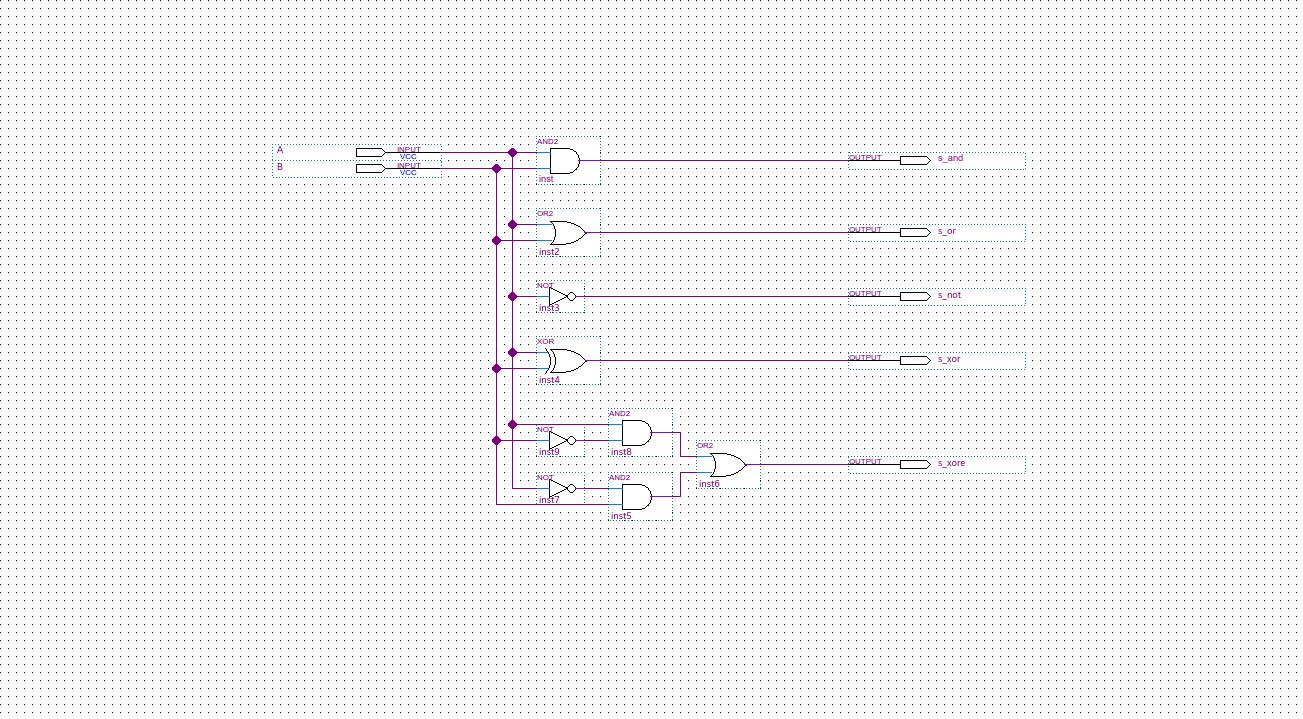
\includegraphics[width=0.9\textwidth]{inciso_a_schematic}
  \caption{Esquema del funcionamiento de las cinco compuertas (Sección A)}
\end{figure}

Tal como se puede apreciar, se tuvieron que agregar algunos elementos 
adicionales. Por una parte, se tienen las señales de entrada:
\begin{itemize}
  \item \textit{A}
  \item \textit{B}
\end{itemize}

Por otra parte, se tienen las salidas:
\begin{itemize}
  \item \textit{s\_and}: La salida de la compuerta AND.
  \item \textit{s\_or}: La salida de la compuerta OR.
  \item \textit{s\_not}: La salida de la compuerta NOT (sólo toma como entrada 
    el valor de \textit{A}).
  \item \textit{s\_xor}: La salida de la compuerta XOR.
  \item \textit{s\_xore}: La salida de la compuerta XOR equivalente.
\end{itemize}

Con lo anterior, se compiló el proyecto. Es importante que el paso anterior se 
llevé a cabo con éxito para que funcione correctamente lo siguiente. Se creó 
un nuevo archivo del tipo \textit{University Program VWF}, a través del cual 
se pudo realizar un \textbf{cronograma} con las señales de entrada y salida de 
simulación. Para llevar a cabo de forma correcta el cronograma, fue importante 
alternar de forma correcta los valores de $A$ y $B$.
\begin{figure}[H]
  \centering
  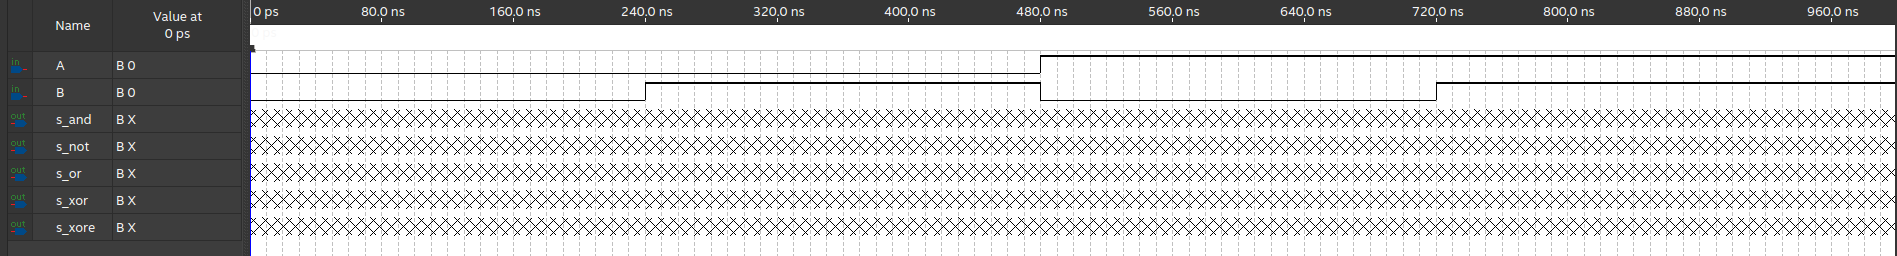
\includegraphics[width=\textwidth]{inciso_a_cron_1}
  \caption{Alternación de los valores de $A$ y $B$ (Sección A)}
  \label{fig:variables_cron_a}
\end{figure}

Al ejecutar la \textit{Simulación Funcional} se obtuvo lo siguiente:
\begin{figure}[H]
  \centering
  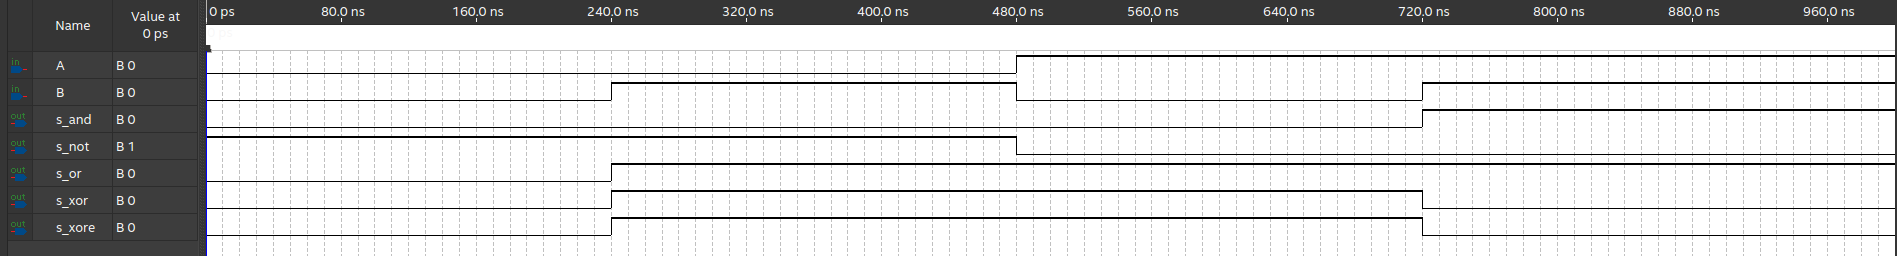
\includegraphics[width=\textwidth]{inciso_a_cron_2}
  \caption{Cronograma del sistema (Sección A)}
  \label{fig:cron_a}
\end{figure}

Se puede comprobar entonces, a través de la Tabla \ref{tab:a_tv} que el 
cronograma de la Figura \ref{fig:variables_cron_a} tiene el comportamiento 
esperodo, por lo tanto, el sistema fue construido de una forma adecuada.

\end{document}
